%%% License: Creative Commons Attribution Share Alike 4.0 (see https://creativecommons.org/licenses/by-sa/4.0/)
%%% Slides are based heavily on earlier versions of this course taught by Jesper Rudiger.

%%% License: Creative Commons Attribution Share Alike 4.0 (see https://creativecommons.org/licenses/by-sa/4.0/)
%%% Slides are based heavily on earlier versions of this course taught by Jesper Rudiger and Peter Norman Sorensen.

\DeclareGraphicsExtensions{.eps, .pdf,.png,.jpg,.mps,}
\usetheme{reMedian}
\usepackage{parskip}
\makeatother

\renewcommand{\baselinestretch}{1.1} 

\usepackage{amsmath, amssymb, amsfonts, amsthm}
\usepackage{enumerate}
\usepackage{hyperref}
\usepackage{url}
\usepackage{bbm}
\usepackage{color}

\usepackage{tikz}
\usepackage{tikzscale}
\newcommand*\circled[1]{\tikz[baseline=(char.base)]{
		\node[shape=circle,draw, inner sep=-20pt] (char) {#1};}}
\usetikzlibrary{automata,positioning}
\usetikzlibrary{decorations.pathreplacing}
\usepackage{pgfplots}
\usepgfplotslibrary{fillbetween}
\usepackage{graphicx}

\usepackage{setspace}
%\thinmuskip=1mu
%\medmuskip=1mu 
%\thickmuskip=1mu 


\usecolortheme{default}
\usepackage{verbatim}
\usepackage[normalem]{ulem}

\usepackage{apptools}
\AtAppendix{
	\setbeamertemplate{frame numbering}[none]
}
\usepackage{natbib}




\title{Financial Markets Microstructure \\ Lecture 3}

\subtitle{Informative Order Flow\\
	Chapter 3.1-3.3 of FPR}

\author{Egor Starkov}

\date{K{\o}benhavns Unversitet \\
	Spring 2020}



\begin{document}
	\frame[plain]{\titlepage}
	\addtocounter{framenumber}{-1}

\section{Revision and problems}

\begin{frame}{What did we do last week?}
\begin{enumerate}
	\item Discuss liquidity
	\item Talk about different measures of spreads
	\begin{itemize}
		\item Quoted
		\item Effective
		\item Realized
	\end{itemize}
	\item Other measures of liqudity(volume etc.)
	\item Estimators for missing data
	\begin{itemize}
		\item Lee-Ready's algorithm for estimating trade direction
		\item Roll's estimator requiring only price data
	\end{itemize}
\end{enumerate}
\end{frame}


\begin{frame}{Exercises}
	\begin{itemize}
		%\item In Absalon, I have attached a commission and fee schedule from Robinhood Financial. More information on \url{www.robinhood.io/}. Discuss the potential effect on other brokerage services.
		\item In this course we mostly imply equity markets. Read the article (on Absalon) about corporate bond markets. Discuss how differences in market structures of stock and bond markets affect liquidity in these markets.
		\item \textcolor{gray}{Recreate the graphs and figures I presented today using the KrispyKreme dataset}
		\item \textcolor{gray}{Solve exercise 8 regarding implementation shortfall, on page 75 in the textbook.
		Discuss the meaning of $m_t$ in this analysis.}
	\end{itemize}
\end{frame}


\begin{frame}{Overview}
	Before we start, let's look at an overview of what we'll do in the rest of the course (weeks = weeks of the course, not calendar weeks)
	
	\textbf{Part 1}: Setting up the models
	\begin{itemize}
	\item \textit{Weeks 3 and 4}: Dealer models 1; \structure{Glosten-Milgrom}, fixed trade size; Bayes' Rule; adverse selection, order costs and inventory risk (\structure{Stoll})
	\item \textit{Week 5}: Dealer models 2; \structure{Kyle}, variable trade size; market depth; estimating liquidity determinants
	\item \textit{Week 6}: Limit order book; \structure{Glosten}: static, random market order demand; market design; \structure{Parlour}: dynamic, endogenous market order demand
	\item \textit{Week 6}: Problem set 1
	\end{itemize}
\end{frame}


\begin{frame}{Overview}
\textbf{Part 2}: Applying the models; topics
\begin{itemize}
	\item \textit{Week 7}: Fragmentation costs, \structure{modified Kyle model}; fragmentation benefits, \structure{modified Glosten LOB model}
	\item \textit{Week 8}: Transparency: search costs, \structure{modified GM model} for order flow transparency
	\item \textit{Weeks 9-10}: Illiquidity premia; liquidity and corporate policy
	\item \textit{Week 10}: Problem set 2
	\item \textit{Week 11}: High-frequency trading; \structure{Biais et al.} 
	\item \textit{Week 12}: Public information; optimal disclosure policies; public announcements and trade volumes
	\item \textit{Weeks 13-14}: Bubbles; herding; common knowledge
	\item \textit{Week 15}: Digital markets
\end{itemize}
\end{frame}


\begin{frame}{Today}
\begin{enumerate}
	\item Go in-depth with the relation between information and prices
	\item What is informational efficiency?
	\item Discuss Glosten and Milgrom's model of information-based trading
	\item Analyze through the model what drives the spread 
\end{enumerate}
\end{frame}



\section{Information and Prices}

\begin{frame}{Motivation}
	Stock prices move around all the time
	\begin{itemize}
		\item Media reports are full of ex post rationalizations 
		\item Look at CNN Money reports (on absalon)
	\end{itemize}
	In this course: everybody agrees on assets' future cash flows ($\approx$value), \textit{conditional} on fundamentals. Broadly speaking two reasons for trading
	\begin{itemize}
		\item \textbf{Risk}: Getting the right risk profile
		\item \textbf{Speculation}: Different expectations of fundamentals because different information
	\end{itemize}
	Different types of information
	\begin{itemize}
		\item \textbf{Public information}:  asset price may move \textit{without} trade
		\item \textbf{Private information} possessed by some traders  $\rightarrow$ reveal this information through their trading
	\end{itemize}
\end{frame}


\begin{frame}{Information and prices}
	\begin{quotation}
		``Fundamentally, in a system in which the knowledge of the relevant facts is dispersed among many people, prices can act to coordinate the separate actions of different people.'' -- \structure{Von Hayek}
	\end{quotation}

	\structure{Fama}'s \textbf{efficient markets hypothesis}: {prices} must be {efficient}.
	\\
	I.e., they must reflect all available information.
\end{frame}


\begin{frame}{Information and prices}
	\centering
	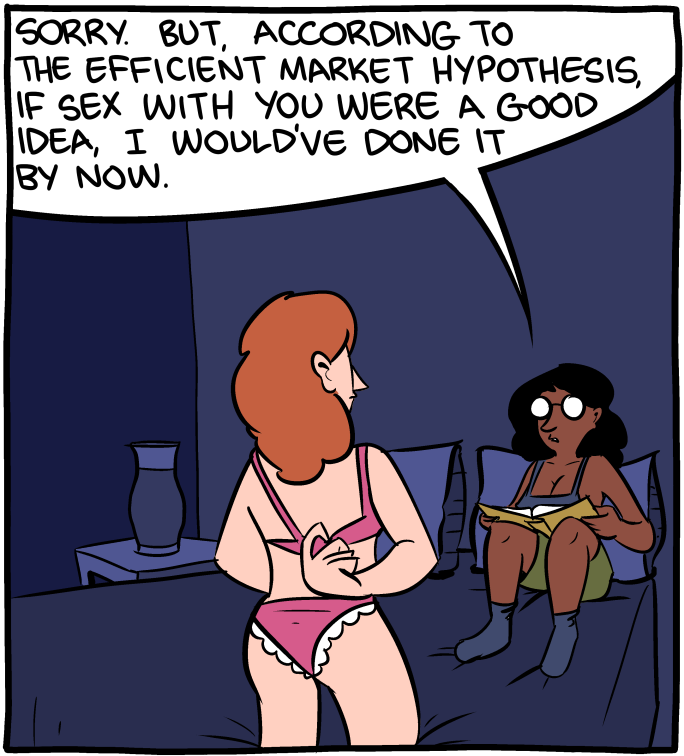
\includegraphics[scale=0.25]{pics/20140603.png}
	
	\url{https://smbc-comics.com}
\end{frame}


\begin{frame}{Information and prices}
	There are different kinds of price efficiency:
	\begin{itemize}
		\item \textbf{Weak form}: Prices reflect historic (price) information
		\item \textbf{Semi-strong form}: Prices reflect all public information
		\item \textbf{Strong form}: Prices reflect all public and private information
	\end{itemize}
\end{frame}


\begin{frame}{Information and prices}
Two counterparts to these views
\begin{itemize}
	\item \textbf{No-trade theorem}: If traders have private information and care only about fundamentals, nobody should ever trade
	\item \textbf{Grossman-Stiglitz (GS) paradox}: 
	\begin{itemize}
		\item Suppose markets were informationally efficient, then prices would reflect traders' private information
		\item Thus: no incentive to acquire information (if this is costly)
	\end{itemize} 
\end{itemize}
\end{frame}


\begin{frame}{Asset value}
	Information: $\Omega_t$ captures the market's (public) knowledge at time $t$ -- ever more is known: 
	\structure{$\Omega_{t+1}=(\Omega_t, I_{t+1})$}. Two approaches:
	\begin{enumerate}
		\item \textbf{Discounted cashflows}: Value at time $t$  = expectation of future cashflows:
		\[
		\mu_t = \mathbb{E}\left[\sum_{s=t}^{\infty} \delta^{t-s} c_s | \Omega_t \right]
		\]
		\item \textbf{Fundamental value}: Value at time $t$ = expectation of underlying fundamental value $v$:
		\[
		\mu_t = \mathbb{E} \left[ v | \Omega_t \right]
		\]
	\end{enumerate}
	Here: use the \structure{fundamental value approach}
\end{frame}


\begin{frame}{Informational efficiency (1)}
\begin{itemize}
	\item Informational efficiency then corresponds to: \structure{$p_t = \mu_t = \mathbb{E}[v|\Omega_t]$}
	\\
	($\Omega_t$ is ``market's knowledge'', so efficiency understood as semi-strong)
	\item Valuation only changes if new information arrives: `innovation in value' is a random variable: \structure{$\epsilon_{t+1} = \mu_{t+1} - \mu_t$}
	\item Then
	\begin{align*}
		\mathbb{E}[\epsilon_{t+1}|\Omega_t] 
		& = \mathbb{E}[\mu_{t+1} - \mu_t|\Omega_t]\\
		& = \mathbb{E}[\mu_{t+1}|\Omega_t] - \mathbb{E}[\mu_t|\Omega_t]\\  
		& = \mathbb{E}[ \mathbb{E}[v|\Omega_{t+1}]|\Omega_t] - \mu_t\\  
		& = \mathbb{E}[v|\Omega_t] - \mu_t\\  
		& = \mu_t- \mu_t\\  
		& = 0.
	\end{align*}
\end{itemize}
\end{frame}


\begin{frame}{Informational efficiency (2)}
	\begin{itemize}
	 \item Also, $\mathbb{E}[\epsilon_{s}\epsilon_t]=0$, $\forall s \ne t$.
	\item Price innovation is equal to the valuation innovation:
	\[
	p_{t+1} - p_t = \mu_{t+1} - \mu_t = \epsilon_{t+1}
	\]
	\item Thus
	\[
	\mathbb{E}[p_{t+1}|\Omega_{t}] = p_t
	\]
	\item When we have informational efficiency, the price is a \alert{martingale}
\end{itemize}
\end{frame}



\section{Glosten and Milgrom (1985)}

\begin{frame}{Glosten and Milgrom (1985)}
	\begin{quotation}
		All models are wrong; some models are useful.
		\begin{flushright}
			-- \structure{George Box}
		\end{flushright}
	\end{quotation}
\end{frame}


\begin{frame}{GM85: Overview}
	\begin{itemize}
		\item The simplest model explaining \structure{spread}.
		\item Spread is driven by adverse selection
		\item Dynamic model, periods $t = 1,2,...$
		\item Two players in every period:
		\begin{itemize}
			\item trader and dealer
			\item dealer long-lived; trader new every period
			\item trader can be informed or not
		\end{itemize}
	\end{itemize}
\end{frame}



\begin{frame}{GM85: Model (1)}
	\textbf{Trader:} is either a speculator or a noise trader, can submit a market order to buy or sell one unit of the asset.
	\begin{itemize}
		\item \structure{Speculator} (probability $\pi$): has private information.
		\begin{itemize}
			\item Risk neutral, chooses his market order $d$ to maximize expected profits:
			\begin{equation*}
				d_t= \left\{
				\begin{aligned}
				1	& \text{ if buy}; \\
				0	& \text{ if abstain}; \\
				-1	& \text{ if sell}.
				\end{aligned}
				\right.
			\end{equation*}
			\item `Hides' behind noise traders
		\end{itemize}
		\item \structure{Noise trader} (probability $1-\pi$): trades for exogenous reasons (hedging, liquidity).
		\begin{itemize}
			\item Buys with fixed probability $\beta_B$; sells w.p. $\beta_S$; abstains w.p. $1-\beta_B - \beta_S$
			\item \alert{Important}: we often assume that these traders behave in a certain way (behavior types) but they can be perfectly rational!
		\end{itemize}
	\end{itemize}
\end{frame}


\begin{frame}{GM85: Model (2)}
	\textbf{Dealer (market maker)}
	\begin{itemize}
		\item Risk neutral
		\item Willing to trade \alert{exactly one unit} (buy/sell/no trade) each period
		\item Quote price before seing trade (limit order)
		\item Does not know whether trader is speculator or noise trader
		\item Sets \alert{bid and ask prices} (for a single unit)
		\item Competitive: prices=expected asset value conditional on information
		\item Trading is sequential: market orders served one by one
	\end{itemize}
\end{frame}


\begin{frame}{Aside on Dealers}
	\begin{quotation}
		\small ``For each security in which a member is registered as a Market Maker, the member shall be willing to buy and sell such security for its own account on a continuous basis during regular market hours and shall enter and maintain a two-sided trading interest (``Two-Sided Obligation'') that is identified to the Exchange as the interest meeting the obligation and is displayed in the Exchange's quotation montage at all times.''
		\begin{flushright}
			-- Nasdaq Rule 4613 (see Absalon)
		\end{flushright}
	\end{quotation}
	\vspace{3ex}
	\begin{quotation}
		\small ``Minimum requirements: at least 85\% of the time, at most 4\% bid-offer
		spread, order size at least worth 4,000 euros''
		\begin{flushright}
			-- Nasdaq OMX Helsinki (see Absalon)
		\end{flushright}
	\end{quotation}
\end{frame}


\begin{frame}{GM85: Model (3)}
\begin{itemize}
	\item \textbf{Asset value}:
	\begin{itemize}
		\item Random asset value $v$ drawn from distribution
		\item Assume $v$ is terminal value (fundamental value)
	\end{itemize}
	\item \textbf{Equilibrium}:
	\begin{itemize}
		\item An equilibrium consists of \structure{bid and ask prices} and \structure{speculator's strategy}
		\item They must be such that: (i) prices are competitive (zero profit for MM), (ii) speculator best-responds to prices (maximizes expected gain).
	\end{itemize}
\end{itemize}
\end{frame}


\begin{frame}{Some questions}
\begin{itemize}
	\item Why are there no uninformed speculators?
	\item What is the role of the dealer?
	\item Why is the dealer willing to trade with better-informed speculators?
\end{itemize}
\end{frame}


\begin{frame}{Analysis. A: Market making}
\begin{itemize}
	\item Dealer quotes bid and ask prices on \textit{one unit}
	\begin{itemize}
		\item Can revise prices between each incoming trade
	\end{itemize}
	\item Quoted ask price $a_t$ only relevant if next incoming trader decides to buy
	\begin{itemize}
		\item Same for bid $b_t$
	\end{itemize}
	\item Risk neutrality and competition implies that the \structure{ask price} and \structure{bid price} are
	\begin{align*}
		a_t & = \mathbb{E}[v|\Omega_{t-1}, Buy]; \\
		b_t &= \mathbb{E}[v|\Omega_{t-1},  Sell].
	\end{align*}
	\item Notice that both sides of the equality depend on prices
\end{itemize}
\end{frame}


\begin{frame}{Analysis. B: Informed trading}
\begin{itemize}
	\item Speculator knows $v$. Given prices $a_t$ and $b_t$, the expected profits $\Pi$ are:
	\begin{equation*}
		\Pi(v,a_t,b_t,d_t)= \left\{
		\begin{aligned}
		&v - a_t  	&& \text{ if } d_t=1; \quad && (Buy)\\
		&0			&&\text{ if } d_t=0; \quad && (Abstain)\\
		&b_t - v 	&& \text{ if } d_t=-1. \quad && (Sell)
		\end{aligned}
		\right.
	\end{equation*}
	\item Speculator is risk-neutral, so his best response to $(a_t,b_t)$ is
	\begin{itemize}
		\item Buy when $v > a_t$, i.e. when $v$ is large enough
		\item Sell when $v<b_t$, i.e. when $v$ is small enough
		\item Abstain if $a_t > v > b_t$
	\end{itemize}
\end{itemize}
\end{frame}


\begin{frame}{Analysis. B: Informed trading (2)}
	\begin{itemize}
		\item The orders reveal information about $v$:
		\begin{align*}
			\mathbb{P}(Buy|\Omega_{t-1}, v) & = (1-\pi) \beta_B + \pi \mathbb{I}(v>a_t) \\
			\mathbb{P}(Sell|\Omega_{t-1}, v)  & = (1-\pi) \beta_S + \pi \mathbb{I}(v<b_t)
		\end{align*}
		In particular, $\mathbb{P}(Buy|\Omega_{t-1}, v)$ is increasing in $v$ (second term is increasing) and $\mathbb{P}(Sell|\Omega_{t-1}, v)$ is decreasing in $v$. Thus:
		\begin{align*}
			a_t & = \mathbb{E}[v|\Omega_{t-1}, Buy] > \mathbb{E}[v|\Omega_{t-1}] = p_{t-1} \\
			b_t & = \mathbb{E}[v|\Omega_{t-1}, Sell] < \mathbb{E}[v|\Omega_{t-1}] = p_{t-1}.
		\end{align*}
		\item Bid-ask spread: $a_t - b_t >0$: this is due to \alert{adverse selection}
	\end{itemize}
\end{frame}


\begin{frame}{Analysis. C: Equilibrium}
	Dealer must make zero profit ({competition}), traders must trade optimally.
	This gives us two \structure{equilibrium conditions}.
	\begin{itemize}
		\item Let $\sigma_t$ denote the speculator's strategy, where $\sigma_t(d_t|v)$ is the probability that the speculator places order $d_t$ if value is $v$
		\item \alert{An equilibrium} consists of \structure{prices $(a_t,b_t)$} and \structure{strategy $\sigma_t$} such that:
		\begin{enumerate}
			\item the ask and bid prices  solve 
			\begin{align*}
			a_t & = \mathbb{E}[v| \Omega_{t-1}, Buy]; \\
			b_t & = \mathbb{E}[v| \Omega_{t-1}, Sell],
			\end{align*}
			given $\sigma_t$
			\item for each $v$, $\sigma_t$ solves 
			\[
			\max_{\sigma_t } \, \{\sigma_t(1|v) [v-a_t] + \sigma_t(-1|v)[b_t-1] \},
			\]
			given $(a_t,b_t)$.
		\end{enumerate} 
	\end{itemize}
\end{frame}


\begin{frame}{Example (as in book)}
\begin{itemize}
	\item \textbf{Single period}: Suppose only one period (drop $t$ subscript, drop $\Omega$)
	\item \textbf{Binary outcome}: $v \in \{ v^H, v^L\}$, with prior $\theta=\mathbb{P}(v^H) $ 
	\item \textbf{Prior value}: What is the prior value of the asset before trading?
	\[
	p=\theta v^H+(1-\theta) v^L.
	\]
	%TODO: check book, p should be mu?
	\item How do we solve? Look for equilibrium with trade. Suppose $v^L < b < a < v^H$. Then speculator buys if $v=v^H$, sells if $v=v^L$
	\item That is, $\sigma(1|v^H)=1$ and $\sigma(-1|v^L)=1$
	\item The procedure is then the following
	\begin{enumerate}
		\item Use the equilibrium conditions from before to calculate prices given the above speculator strategy
		\item Check that these prices satisfy $v^L < b < a < v^H$
	\end{enumerate}
\end{itemize}
\end{frame}


\begin{frame}{Example (2)}
\begin{itemize}
	\item Let's solve for the ask price. First:
	\begin{align*}
		\mathbb{P}(Buy| v^H) & = (1-\pi) \beta_B + \pi \\
		\mathbb{P}(Buy| v^L) & = (1-\pi) \beta_B
	\end{align*}
	Then by Bayes' Rule
	\begin{align*}
		\mathbb{P}(v^H|Buy) & = \frac{\mathbb{P}(v^H) \mathbb{P}(Buy| v^H)}{\mathbb{P}(Buy)}  \\
		& = \frac{\theta [(1-\pi)\beta_B+\pi]}{(1-\pi)\beta_B+ \pi\theta}  \\
		& =  \theta + \frac{\theta(1-\theta) \pi}{(1-\pi)\beta_B+\pi\theta}
	\end{align*}
\end{itemize}
\end{frame}


\begin{frame}{Example (3)}
\begin{itemize}
	\item The ask price is the expected value, given a buy order:
	\begin{align*}
		a 
		& = \mathbb{P}(v^H| Buy) v^H + [1-\mathbb{P}(v^H| Buy)] v^L \\
		& = \left[ \theta + \frac{\theta(1-\theta) \pi}{(1-\pi)\beta_B+\pi\theta} \right] v^H + \left[ 1 - \left( \theta + \frac{\theta(1-\theta) \pi}{(1-\pi)\beta_B+\pi\theta} \right) \right] v^L\\
		& = p + \frac{\theta(1-\theta) \pi}{(1-\pi)\beta_B+\pi\theta} (v^H -v^L).
	\end{align*}
	\item Doing a similar exercise for $b$ we find
	\begin{align*}
		a - p 		&= \frac{\theta(1-\theta) \pi}{(1-\pi)\beta_B+\pi\theta}(v^H-v^L) \\
		p - b 		&= \frac{\theta(1-\theta) \pi}{(1-\pi)\beta_S+\pi(1-\theta)}(v^H-v^L)
	\end{align*}
\end{itemize}
\end{frame}


\begin{frame}[label=example]{Example (4)}
\begin{itemize}
	\item Notice: $a$ rises in $\pi$, falls with $\beta_B$ (book considers $\beta_B=1/2$)
	\item Add the two expressions to get bid-ask spread $S = a-b$
	\begin{itemize}
		\item If $\beta_B=\beta_S=1/2$, spread is increasing in $\theta(1-\theta)$
		\item i.e. spread higher when dealer faces greater initial uncertainty about $v$
	\end{itemize}
	\item Finally, we must check that our assumption holds: easy to check that $v^H > a > b > v^L$. Hence, \alert{this is an equilibrium}
	\item \structure{Price discovery}: Return to multiperiod setting. Each order conveys information, dealers learn, and 
	\center
	$p_t \rightarrow v$
	\hyperlink{dynamics}{\beamerbutton{Dynamics}}
\end{itemize}
\end{frame}


\begin{frame}{Simulation}
	Dealer beliefs: Each curve shows the evolution of dealer's beliefs in each run (10 runs of 100 orders)
	\quad
	\center
	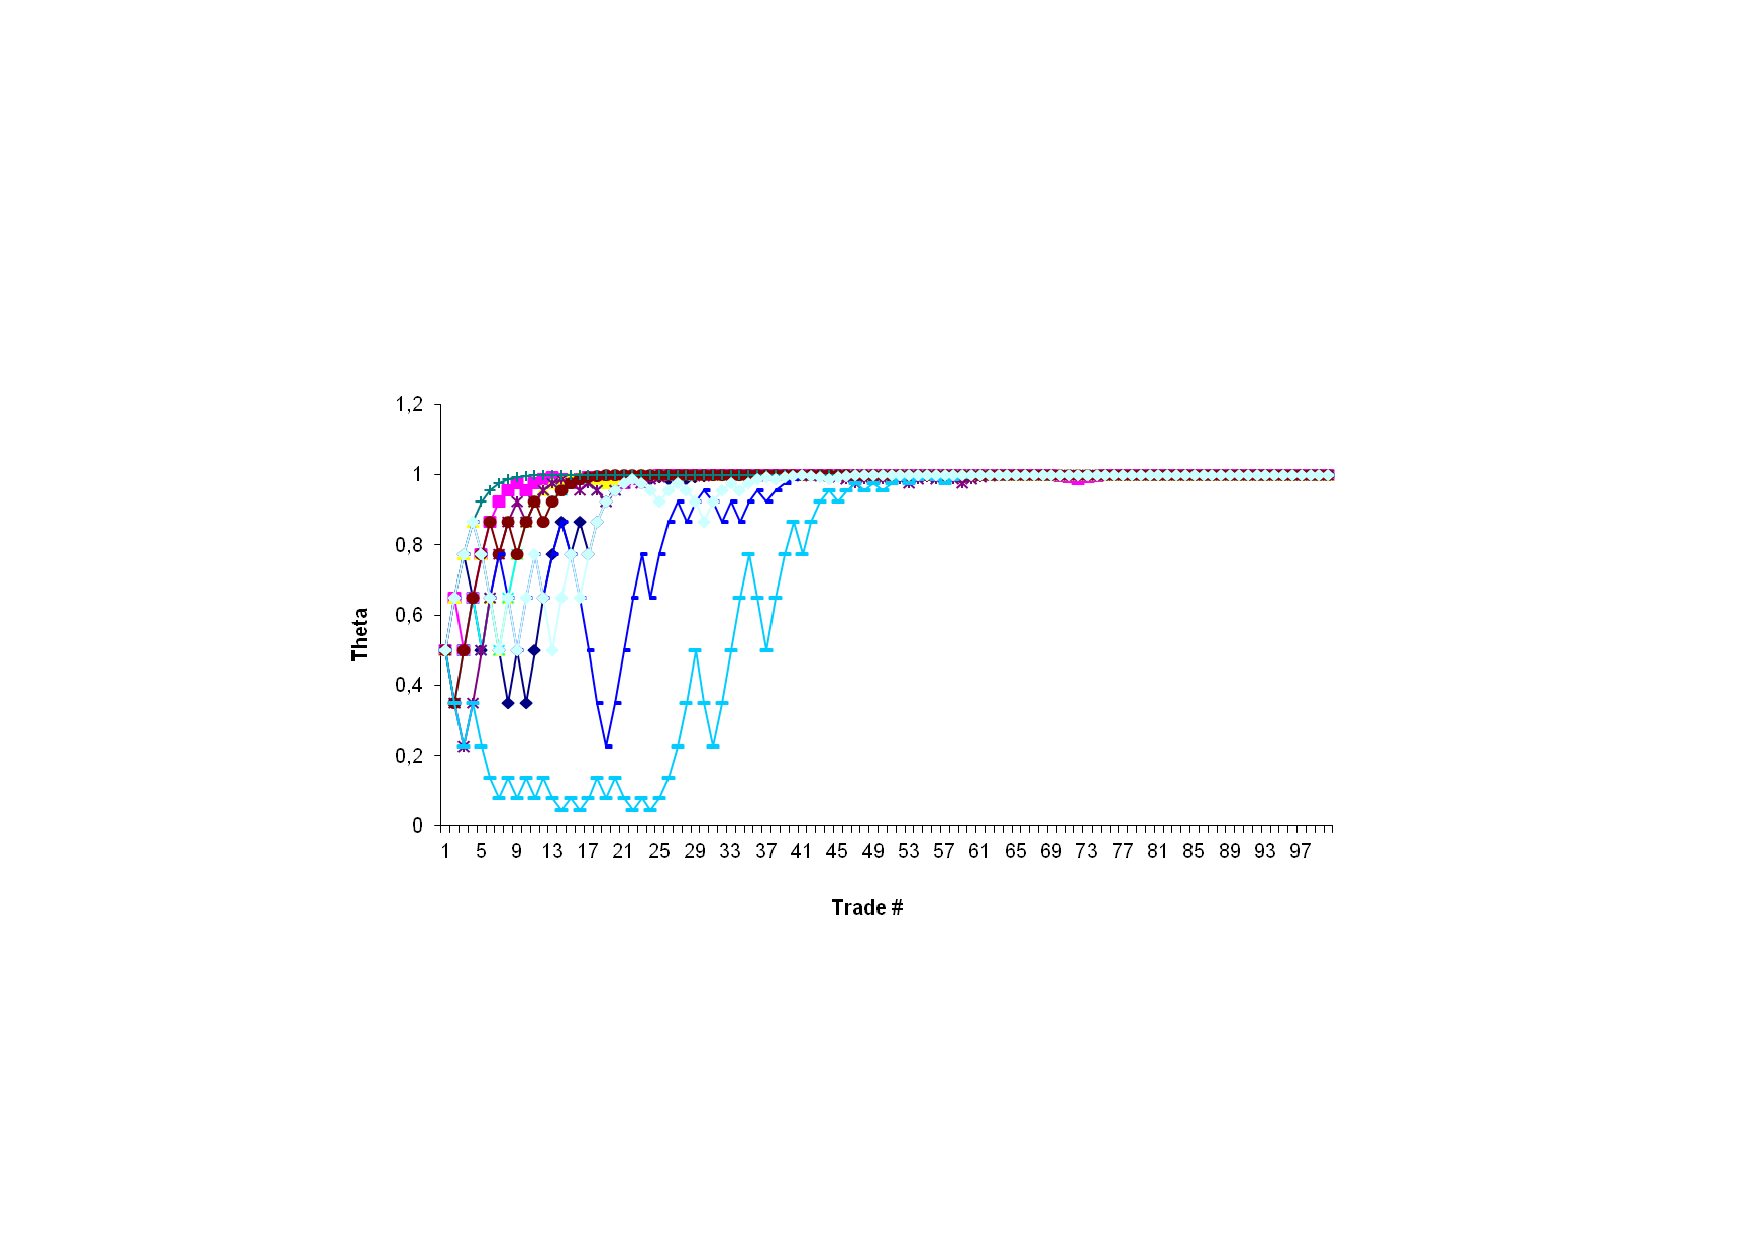
\includegraphics[width=1\linewidth]{pics/DealerBeliefs_Image.pdf}
\end{frame}


\begin{frame}{Model overview: Glosten and Milgrom}
	\structure{Model}
	\begin{itemize}
		\item \textbf{Dealer model}: Prices are set each period, discriminative, normally competitive (zero profits)
		\item \textbf{Non-market clearing}: Only one unit traded  - not market clearing (traders may wish to buy/sell more)
		\item Only \textbf{fundamental value} matters,  no speculation/resale
	\end{itemize}
	\structure{Discussion}
	\begin{itemize}
		\item \textbf{Insights}: Adverse selection as a driver of the spread
		\item \textbf{Shortcomings}: Trade fixed amount, trade once, no resale
		\item \textbf{Advantages}: (Relatively) simple analysis, flexible, trader is not price-taker (realizes price-impact)
	\end{itemize}
\end{frame}


\begin{frame}{Summary}
	What did we learn from the Glosten and Milgrom model?
	\begin{enumerate}
		\item Information, prices and the spread
		\begin{itemize}
			\item Prices will reflect the information revealed by trades
			\item The spread is increasing in informational asymmetry (adverse selection) and in uncertainty about asset value
		\end{itemize}
		\item Informational efficiency
		\begin{itemize}
			\item Prices are always semi-strong efficient, in the long run also strong-form efficient
		\end{itemize}
		\item Noise trading
		\begin{itemize}
			\item Noise trading keeps the market liquid and improves spreads
			\item Informed speculation increases spreads, but improves price discovery - dilemma for regulators
		\end{itemize}
	\end{enumerate}
\end{frame}


\begin{frame}{Questions for next week}
	\begin{itemize}
		%\item See next page for a text from The Securities and Exchange Commission on insider trading, from its homepage \url{http://www.sec.gov/answers/insider.htm}. Discuss potential restrictions in the definition.
		\item FPR chapter 3 exercises (p. 124-125):
		\begin{itemize}
			\item exercise 2 -- solve GM model with numbers instead of letters
			\item exercise 3 about the GM model where speculators are not perfectly informed, but instead receive a signal about the value of the asset
		\end{itemize}
	\end{itemize}
\end{frame}


%\begin{frame}{Questions for next week (2)}
%	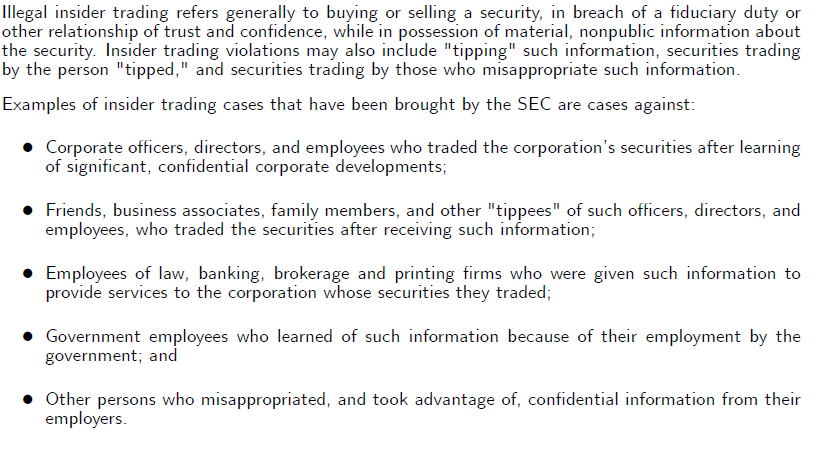
\includegraphics[width=1\linewidth]{pics/InsiderTrading_Text}
%\end{frame}


\begin{frame}<handout:0>[label=dynamics]
	\frametitle{Dynamics}
	Suppose we are in the simple binary model with the following parameters
	\begin{itemize}
		\item Probability of informed speculators: $\pi = 0.3$
		\item Probability (ex ante) of high value: $\theta = 0.5$
		\item $v^H=150$ and $v_L=100$
	\end{itemize}
	Consider 12 periods, with the following sequence of buys (b) and sells (s)
	\[
	ssbssssssssss
	\]
\end{frame}


\begin{frame}
	\frametitle{Dynamics}
	First period: sell
	\center
	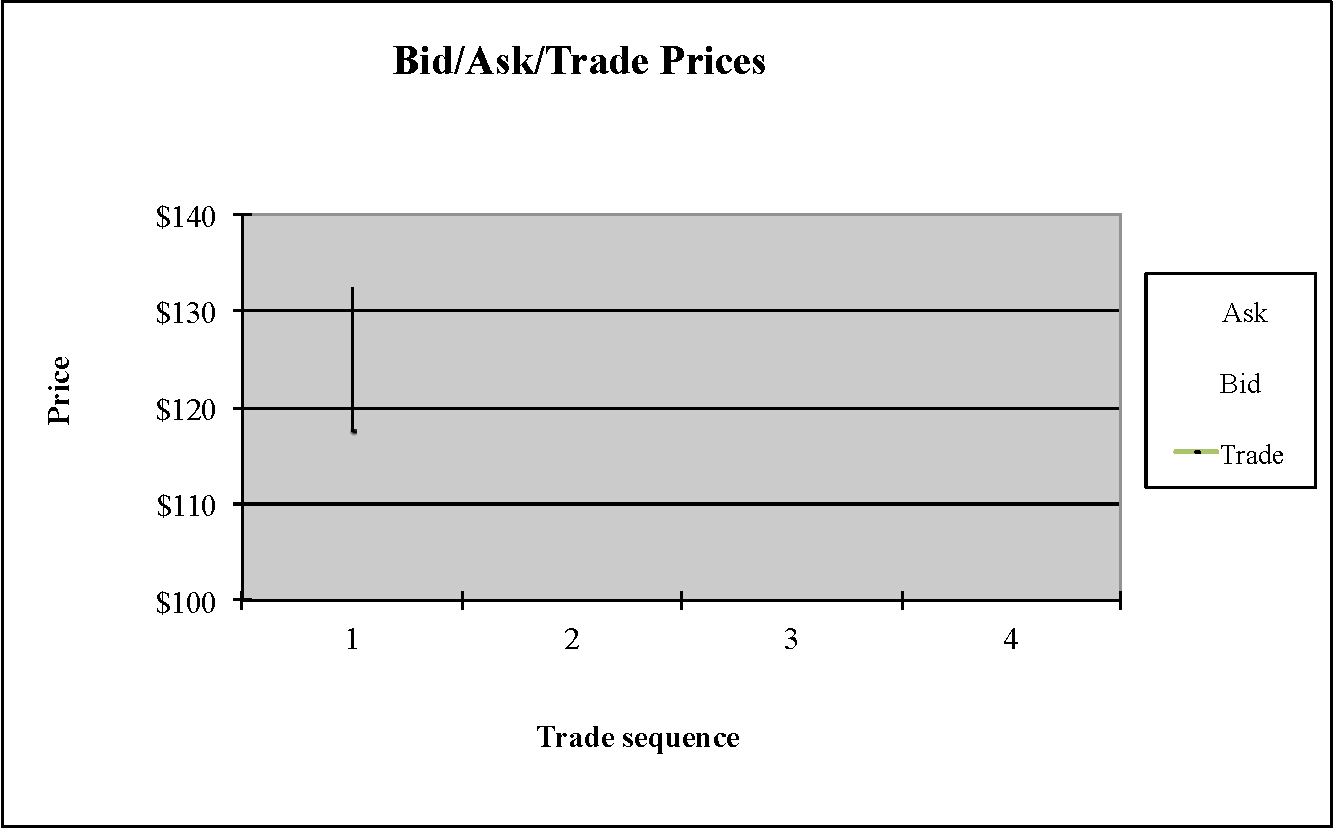
\includegraphics[width=0.9\linewidth]{pics/P1_Image.pdf}
\end{frame}


\begin{frame} [noframenumbering]
	\frametitle{Dynamics}
	Second period: sell
	\center
	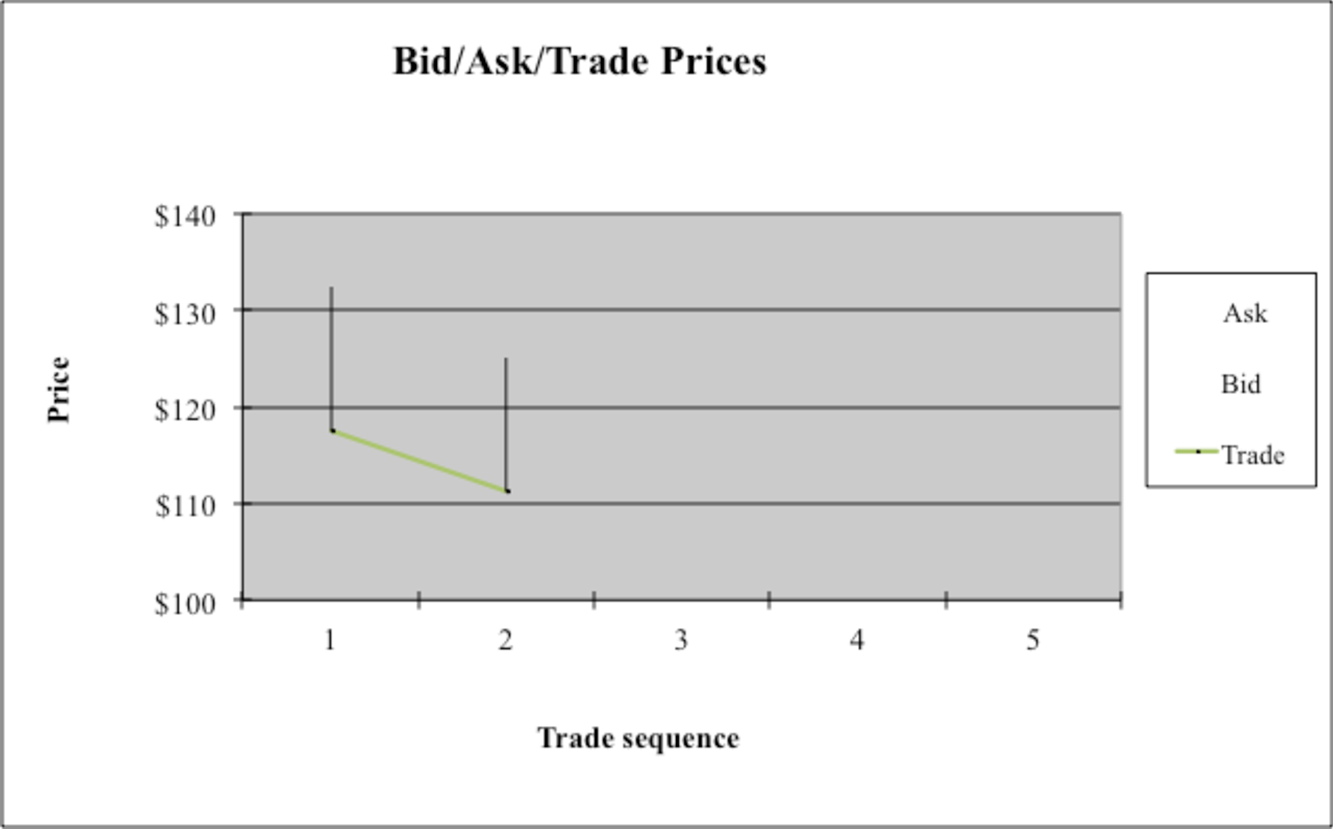
\includegraphics[width=0.9\linewidth]{pics/P2_Image.pdf}
\end{frame}


\begin{frame} [noframenumbering]
	\frametitle{Dynamics}
	Third period: buy
	\center
	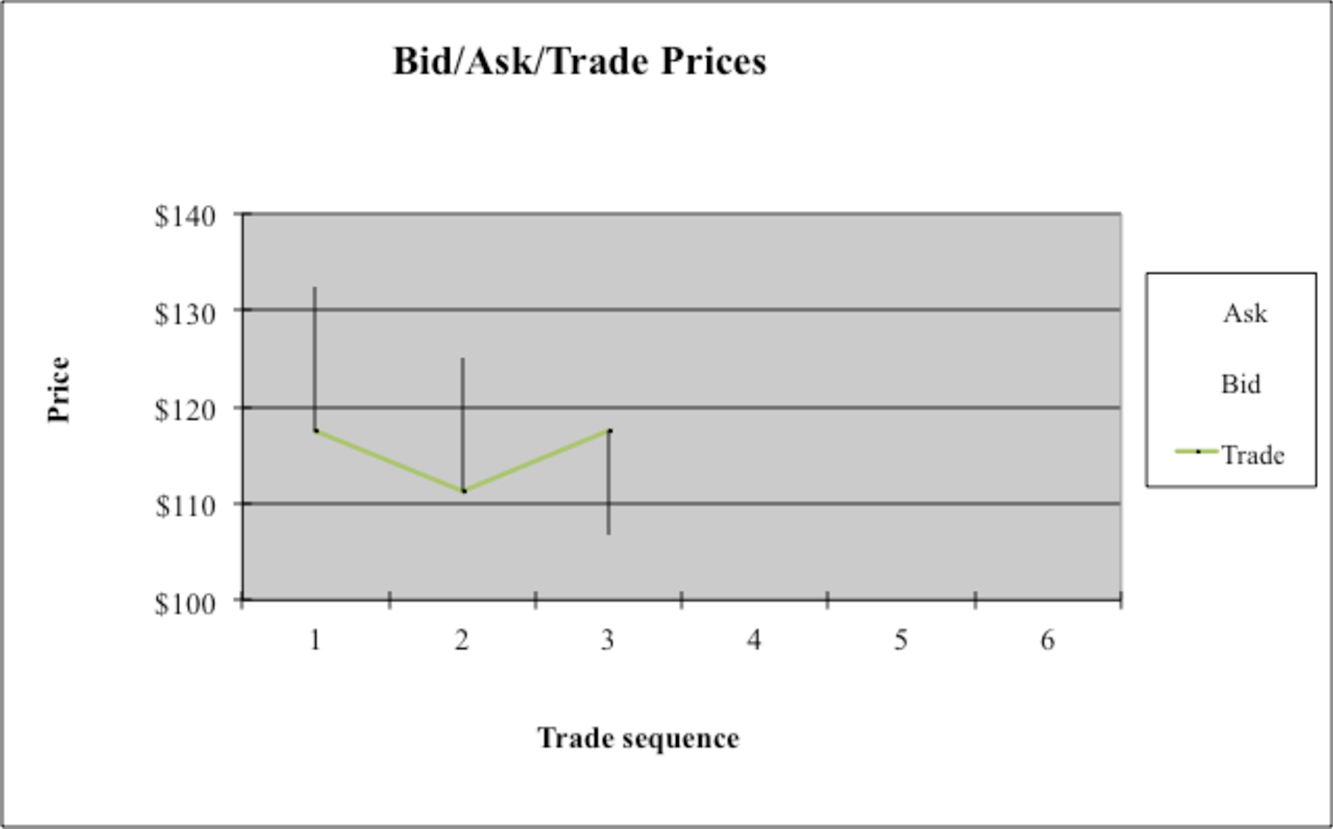
\includegraphics[width=0.9\linewidth]{pics/P3_Image.pdf}
\end{frame}


\begin{frame} [noframenumbering]
	\frametitle{Dynamics}
	Fourth period: sell
	\center
	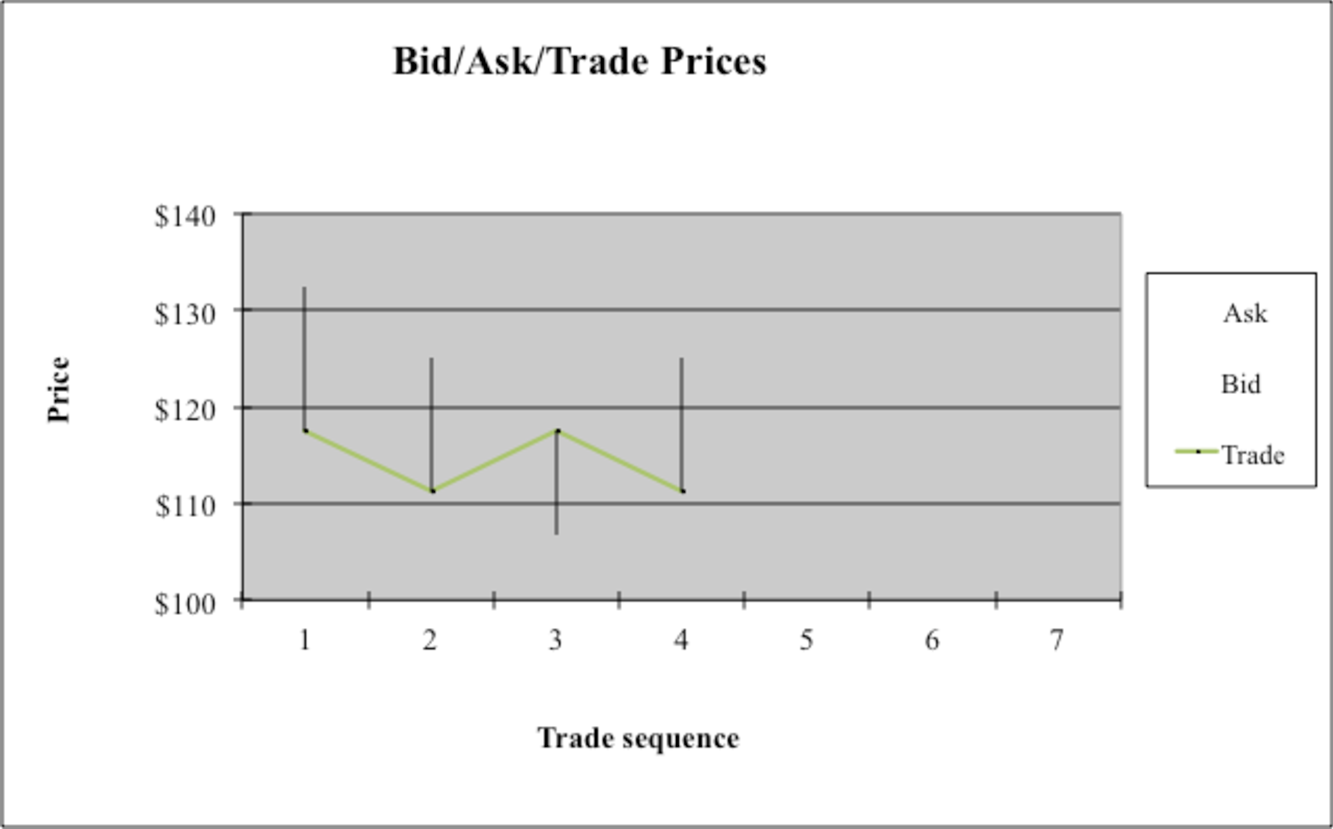
\includegraphics[width=0.9\linewidth]{pics/P4_Image.pdf}
\end{frame}


\begin{frame} [noframenumbering]
	\frametitle{Dynamics}
	Fifth period: sell
	\center
	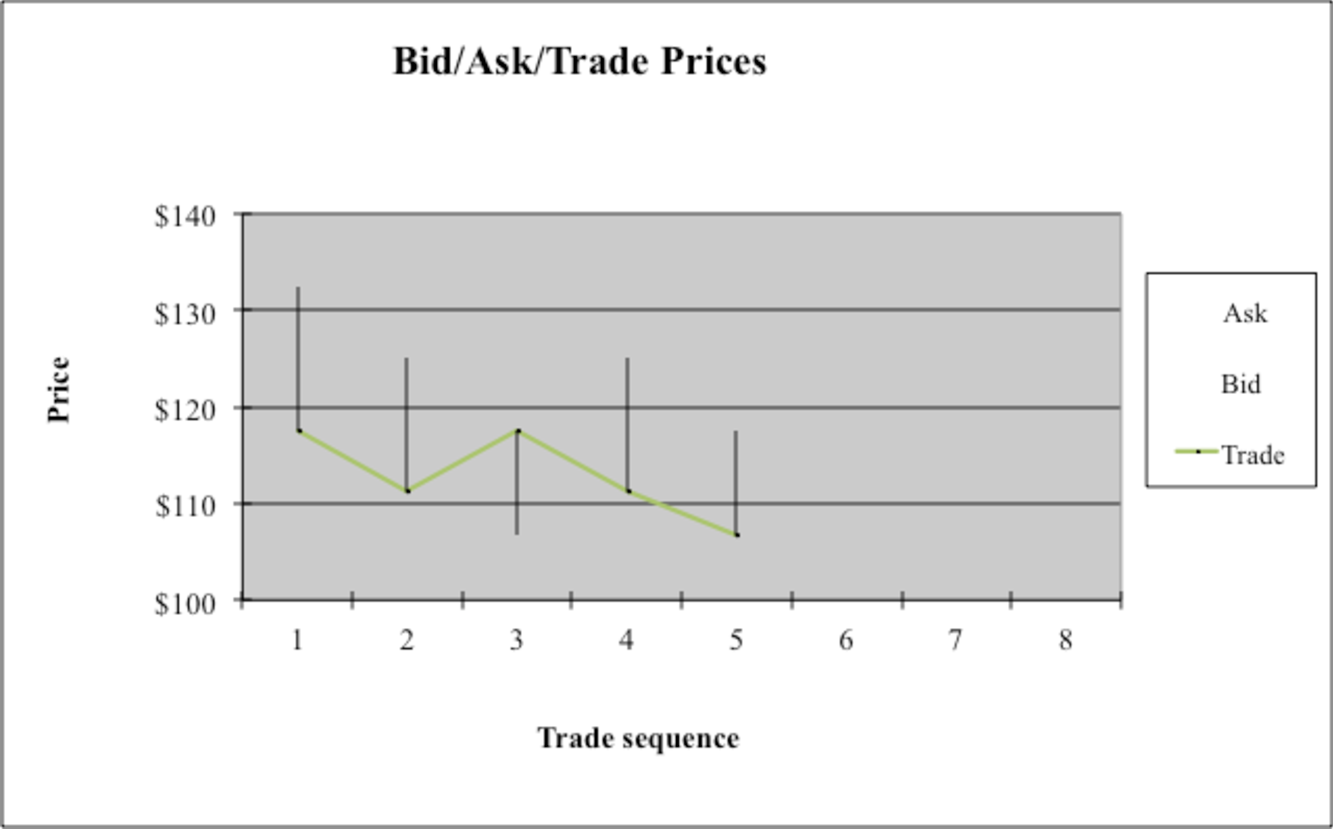
\includegraphics[width=0.9\linewidth]{pics/P5_Image.pdf}
\end{frame}


\begin{frame} [noframenumbering]
	\frametitle{Dynamics}
	Sixth period: sell
	\center
	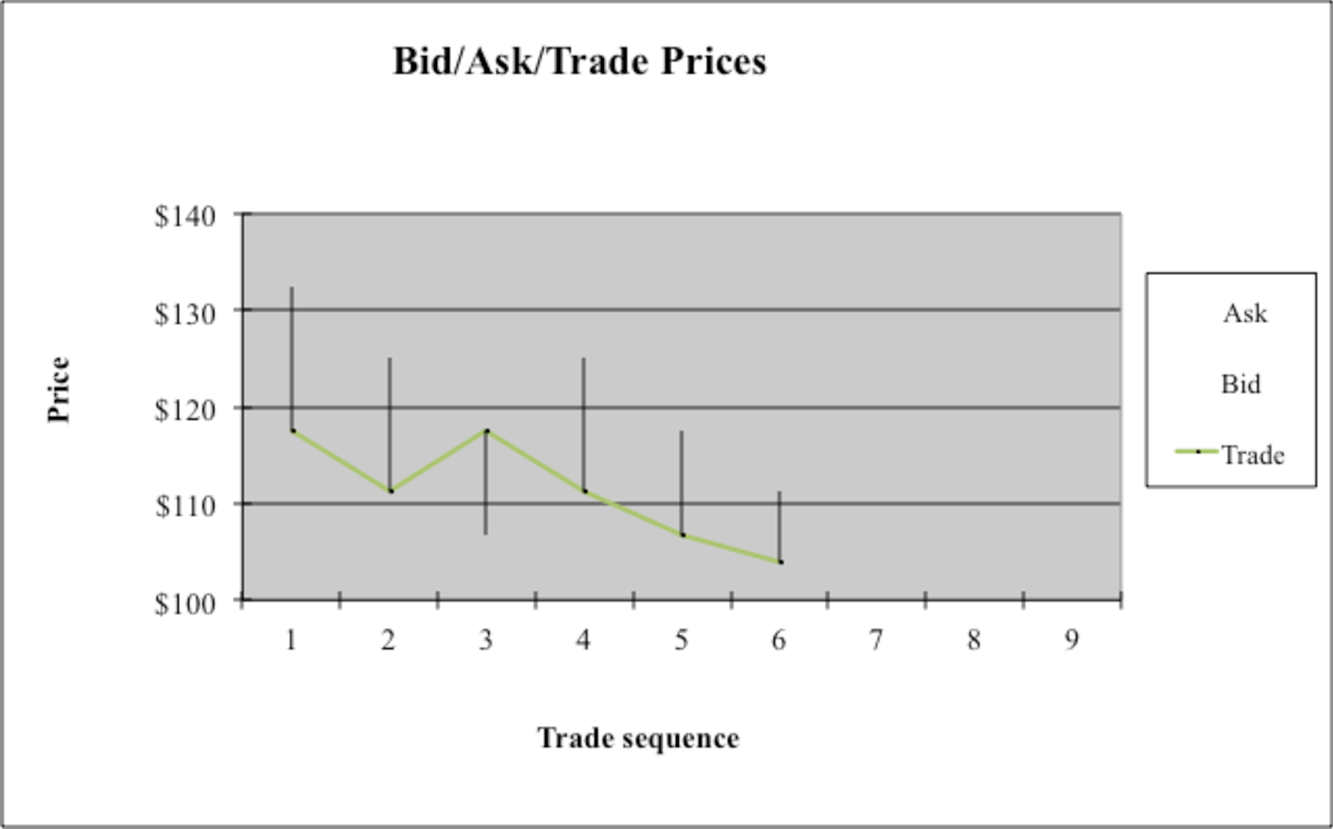
\includegraphics[width=0.9\linewidth]{pics/P6_Image.pdf}
\end{frame}


\begin{frame} [noframenumbering]
	\frametitle{Dynamics}
	Seventh period: sell
	\center
	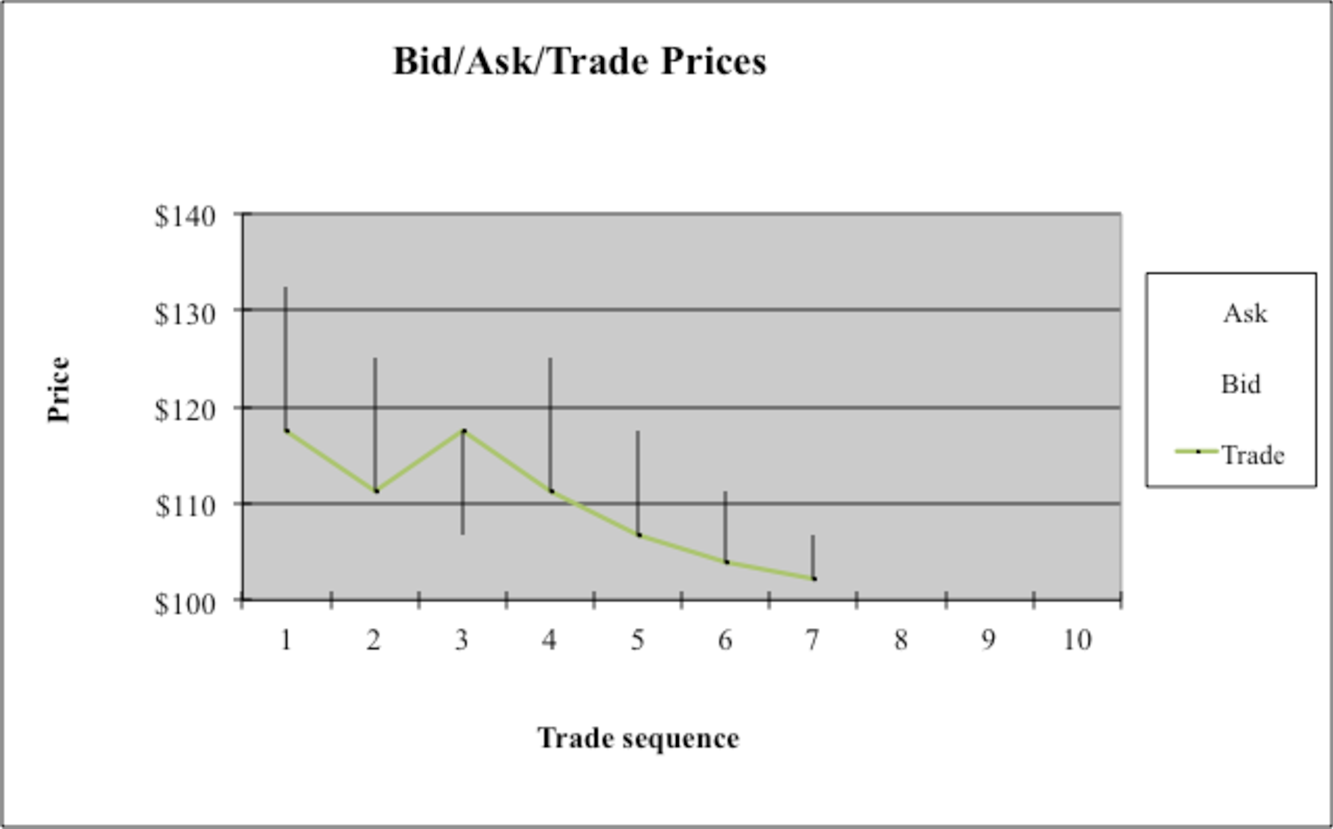
\includegraphics[width=0.9\linewidth]{pics/P7_Image.pdf}
\end{frame}


\begin{frame} [noframenumbering]
	\frametitle{Dynamics}
	Eigth period: sell
	\center
	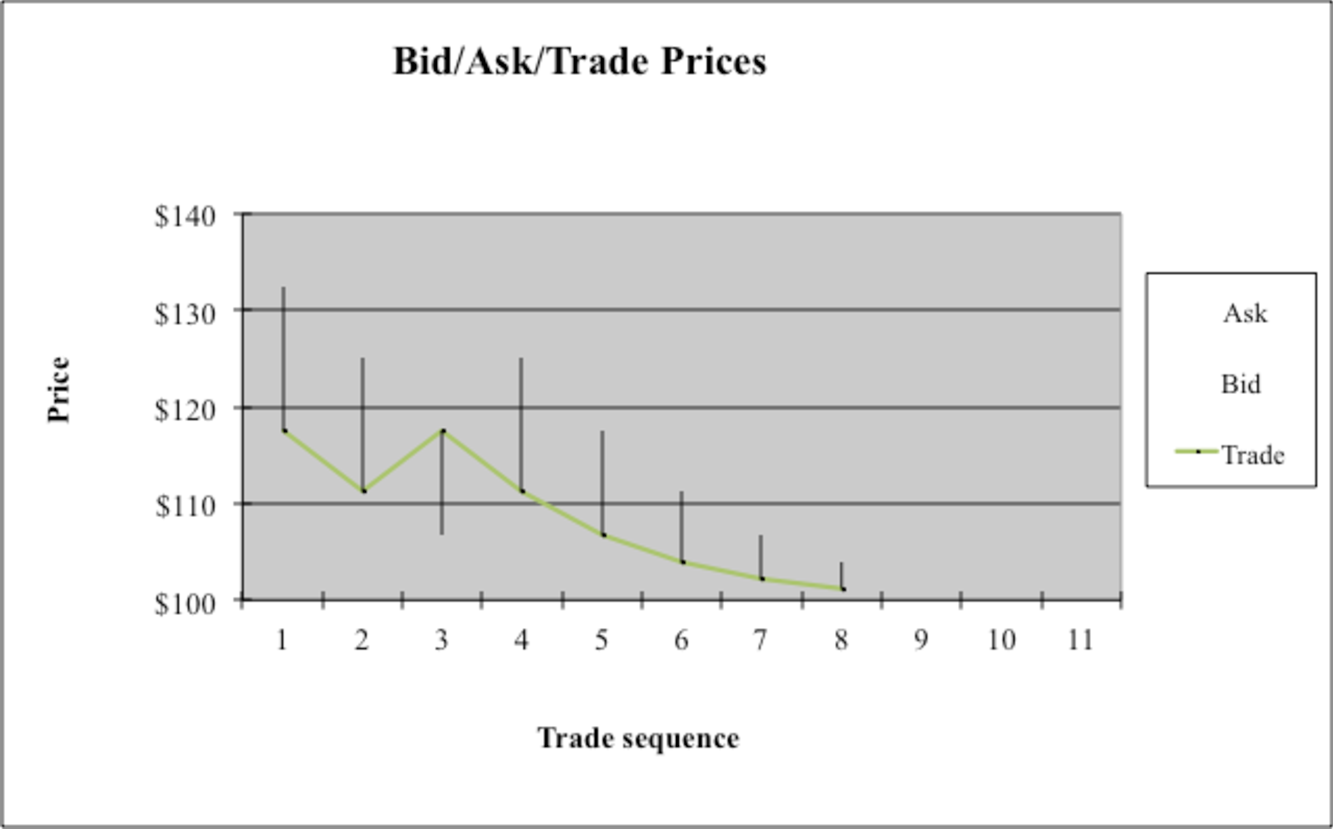
\includegraphics[width=0.9\linewidth]{pics/P8_Image.pdf}
\end{frame}


\begin{frame} [noframenumbering]
	\frametitle{Dynamics}
	Ninth period: sell
	\center
	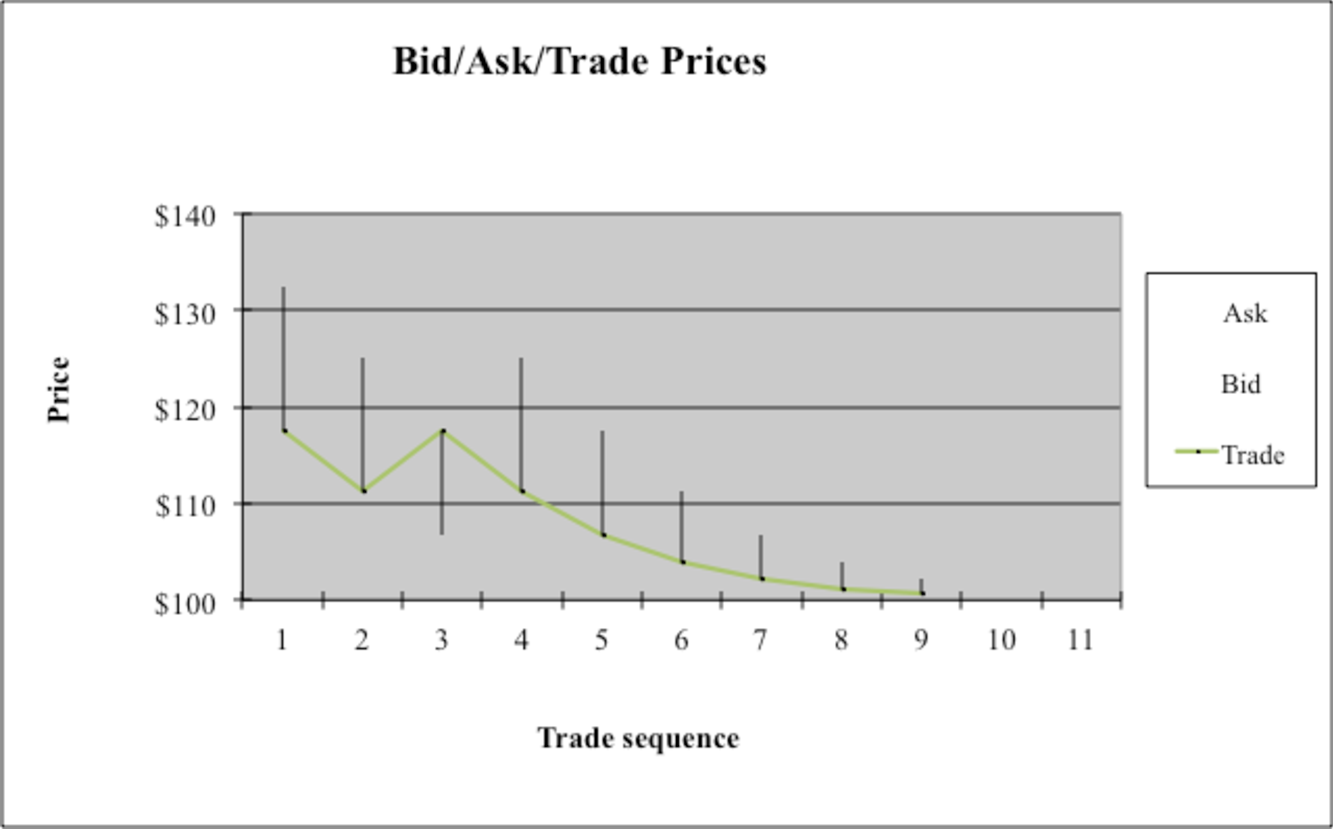
\includegraphics[width=0.9\linewidth]{pics/P9_Image.pdf}
\end{frame}


\begin{frame} [noframenumbering]
	\frametitle{Dynamics}
	Tenth period: sell
	\center
	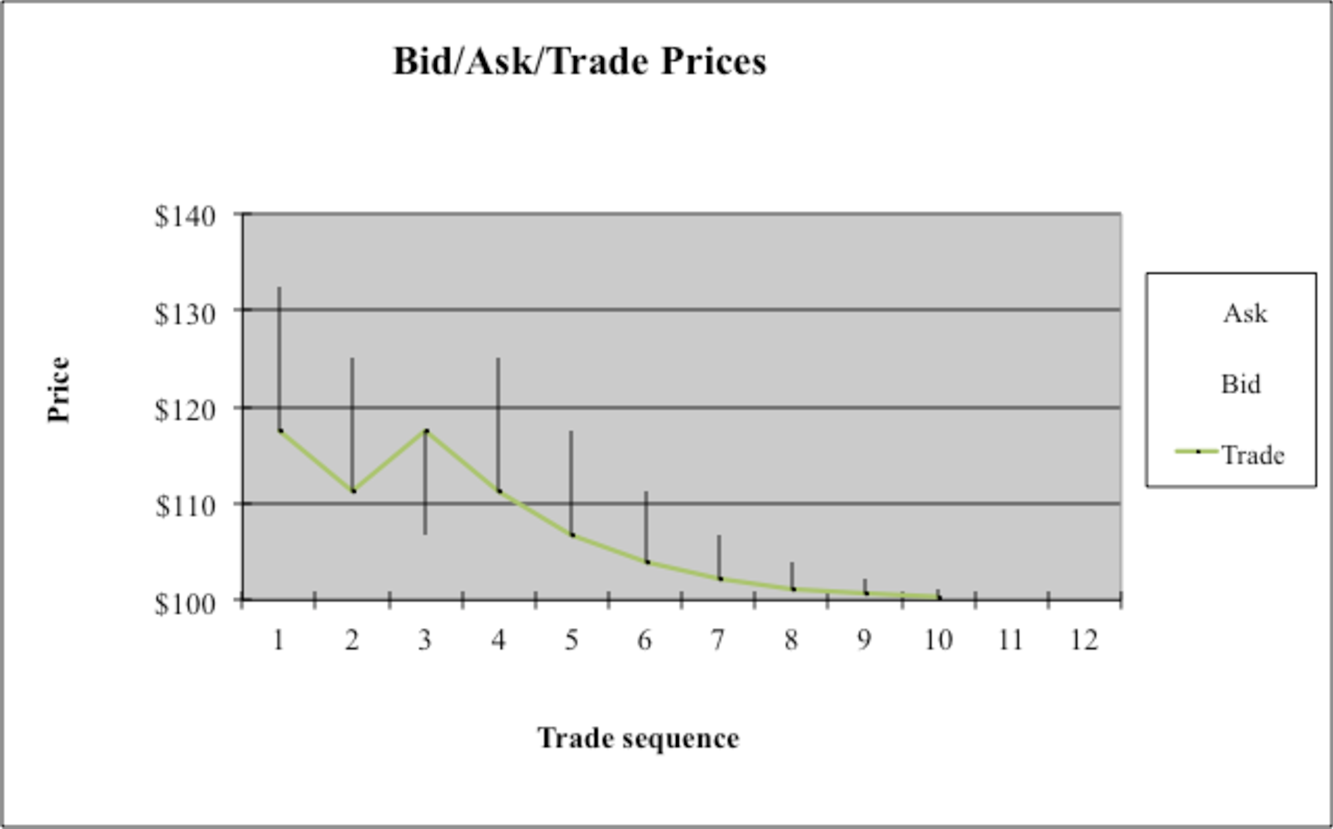
\includegraphics[width=0.9\linewidth]{pics/P10_Image.pdf}
\end{frame}


\begin{frame} [noframenumbering]
	\frametitle{Dynamics}
	Eleventh period: sell
	\center
	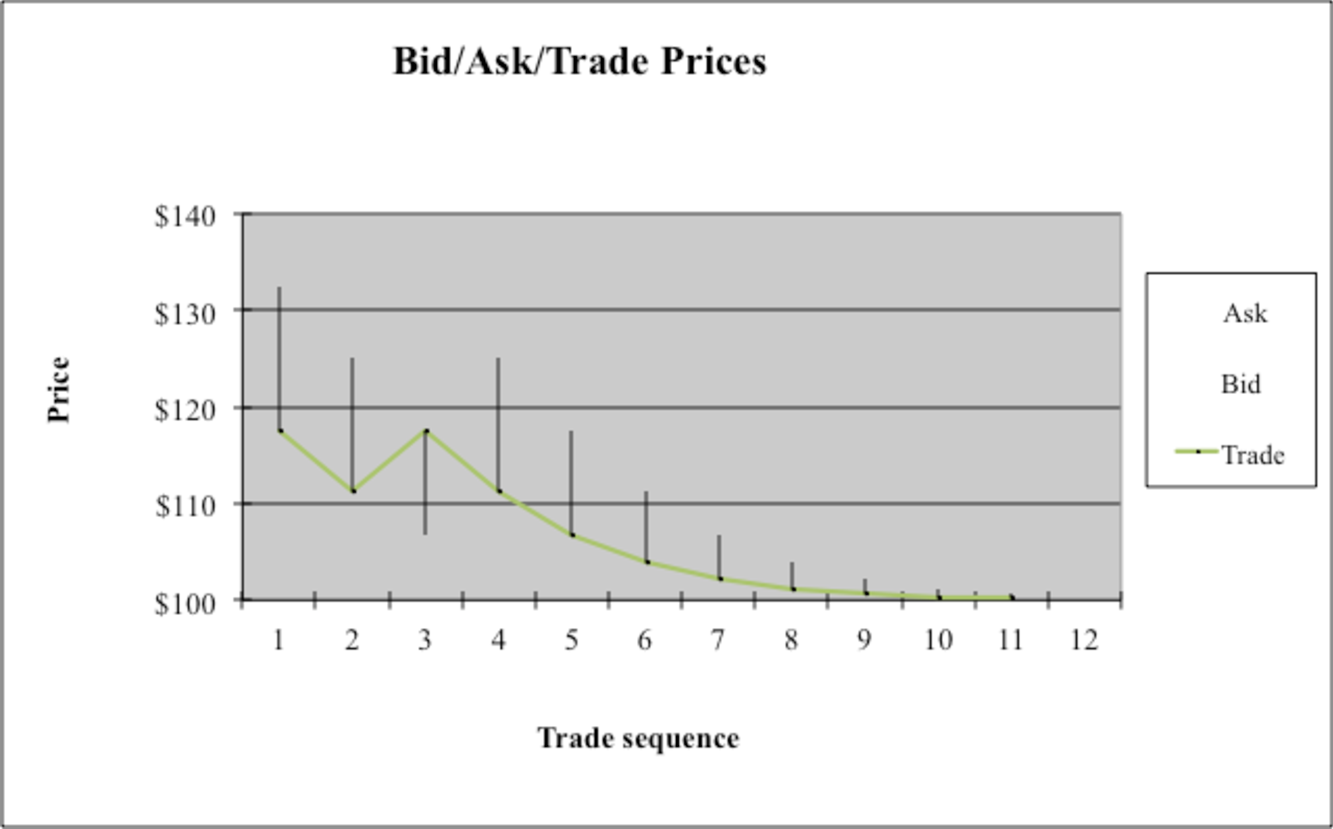
\includegraphics[width=0.9\linewidth]{pics/P11_Image.pdf}
\end{frame}


\begin{frame} [noframenumbering]
	\frametitle{Dynamics}
	Twelfth period: sell
	\center
	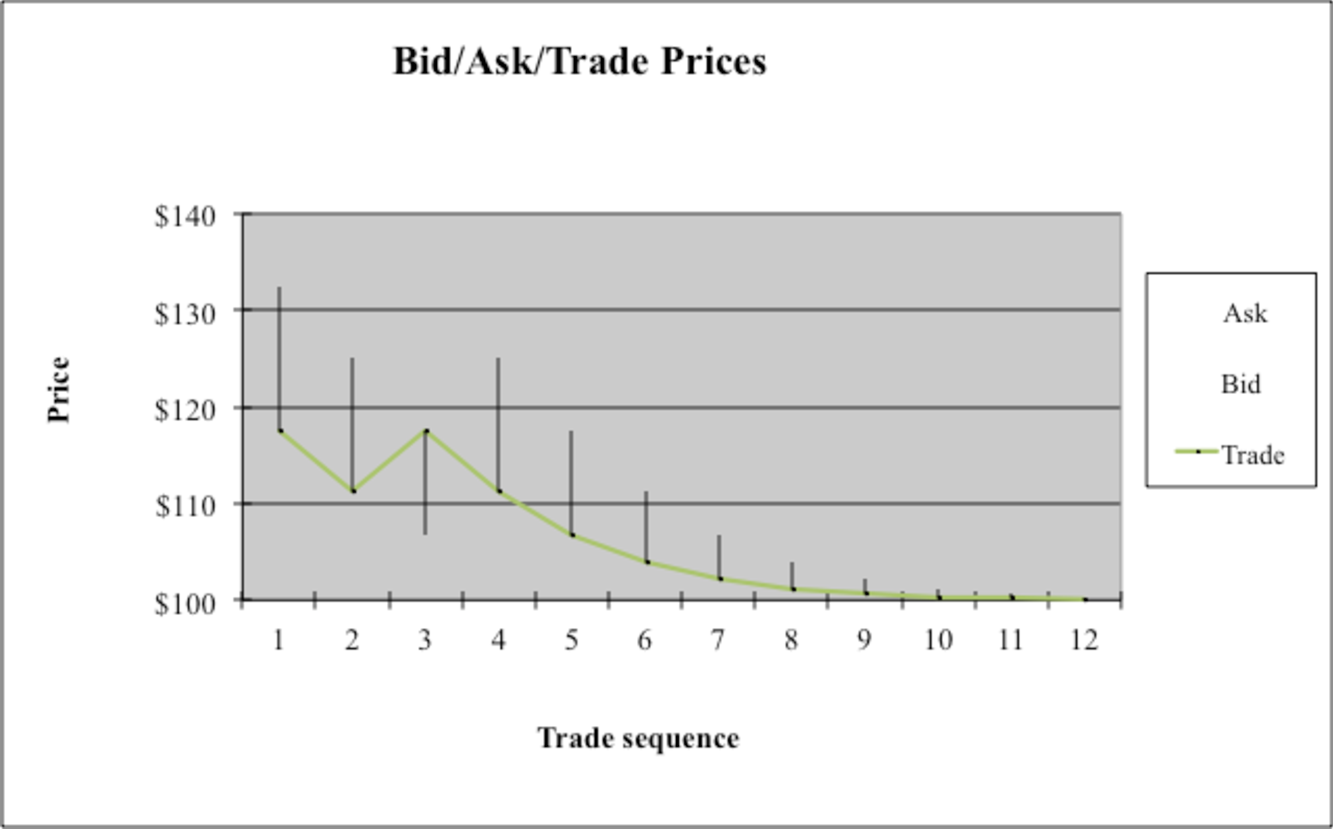
\includegraphics[width=0.9\linewidth]{pics/P12_Image.pdf}
\end{frame}


\begin{frame} [noframenumbering]
	\frametitle{Dynamics}
	Let's consider an alternative case:
	\[
	bbbsssssssss
	\]
	Here we have a spell of buying in the beginning, before a long series of selling
\end{frame}


\begin{frame} [noframenumbering]
	\frametitle{Dynamics}
	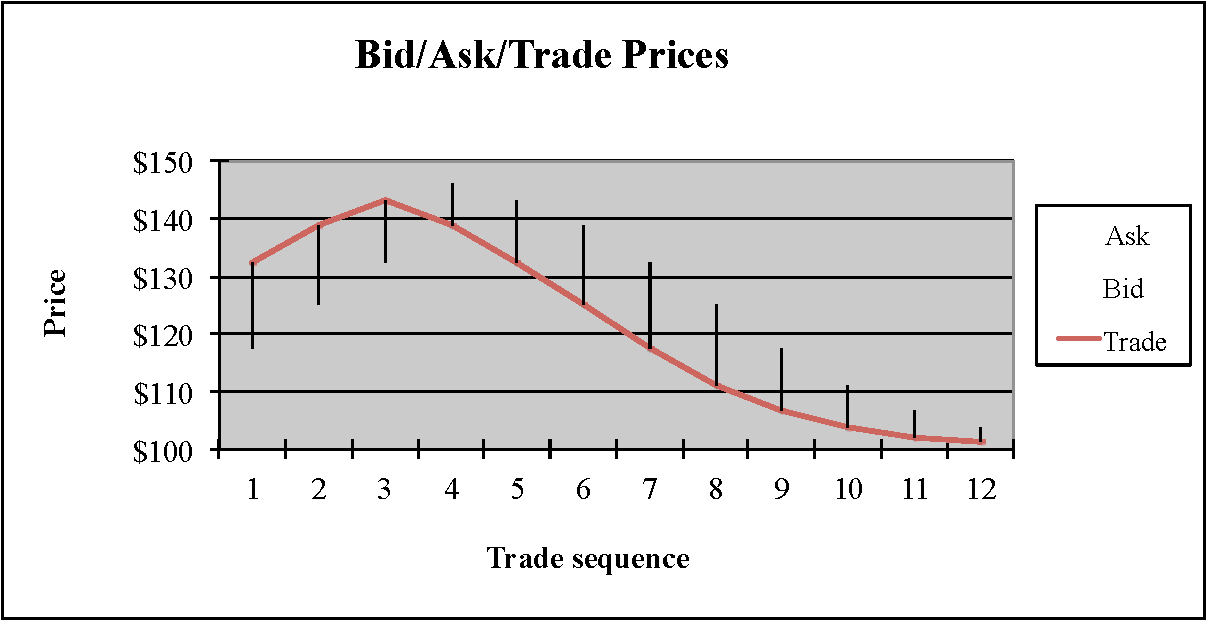
\includegraphics[width=1\linewidth]{pics/Bubble_Image.pdf}
	\hyperlink{example}{\beamerbutton{back}}
\end{frame}


\end{document} 